\section{Gadgets}
\label{gadgets}


% { \tt Gadget}( $\left\langle \text{Input} \right\rangle, \left\langle \text{Output}  \right\rangle$ )

\newcommand{\warpunit}{{\tt Warp\_Unit}}
\newcommand{\prewarp}{{\tt Pre\_Warp}}
\newcommand{\firstwarp}{{\tt First\_Warp}}
\newcommand{\warpbridge}{{\tt Warp\_Bridge}}
\newcommand{\secondwarp}{{\tt Second\_Warp}}
\newcommand{\postwarp}{{\tt Post\_Warp}}

\newcommand{\dtop}{{\tt Digit\_Top}}
\newcommand{\dwriter}{{\tt Digit\_Writer}}
\newcommand{\dreader}{{\tt Digit\_Reader}}

\newcommand{\returnfromdonereadnextrow}{{\tt Return\_From\_Digit1\_Read\_Next\_Row}}
\newcommand{\returnfromdtworeadnextrow}{{\tt Return\_From\_Digit2\_Read\_Next\_Row}}
\newcommand{\returnfromdthreereadnextrow}{{\tt Return\_From\_Digit3\_Read\_Next\_Row}}

\newcommand{\returnfromdonereaddtwo}{{\tt Return\_From\_Digit1\_Read\_Digit2}}
\newcommand{\returnfromdonereaddtwocasetwo}{{\tt Return\_From\_Digit1\_Read\_Digit2\_Case2}}
\newcommand{\returnfromdtworeaddthree}{{\tt Return\_From\_Digit2\_Read\_Digit3}}
\newcommand{\returnfromdthreereaddone}{{\tt Return\_From\_Digit3\_Read\_Digit1}}

\newcommand{\inc}{{\tt carry}}

\newcommand{\dtopdonecasetwo}{{\tt Digit\_Top\_Digit1\_Case2}}
\newcommand{\dtopdtwocasetwo}{{\tt Digit\_Top\_Digit2\_Case2}}
\newcommand{\dtopdthreecasethree}{{\tt Digit\_Top\_Digit3\_Case3}}

% todo: fix wording
When describing a special cases, i.e. ``case $x$ - digit $y$'', whatever follows
will only apply to the MSR (due to each case only affecting the MSR.)

\subsection{ Counter Unit }




    \subsubsection{ Digit readers }

    % For each digit length L
    \subsubsection{ Warping }

    % For each index in 1, 2, 3, and carry in 0,1
        For each $d \in \{0, 1\}^l$, $i = 1, 2, 3$

        \begin{enumerate}[label={--}]

            \item $\prewarp   (\langle d, i, \inc\rangle)\approx O(1)$
                \begin{figure}[H]
                    \begin{subfigure}[t]{0.2\textwidth}
                        \centering
                        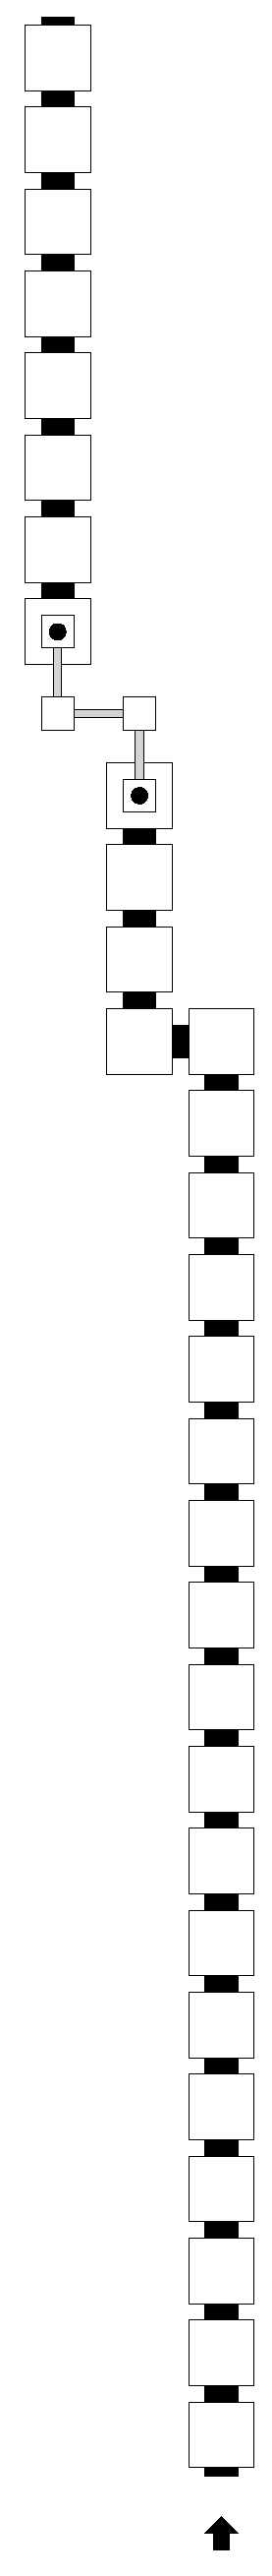
\includegraphics[width=0.2\textwidth]{warping/pre_warp_general}
                        \caption{\label{fig:warping/pre_warp_general} General }
                    \end{subfigure}%
                    ~
                    \begin{subfigure}[t]{0.2\textwidth}
                        \centering
                        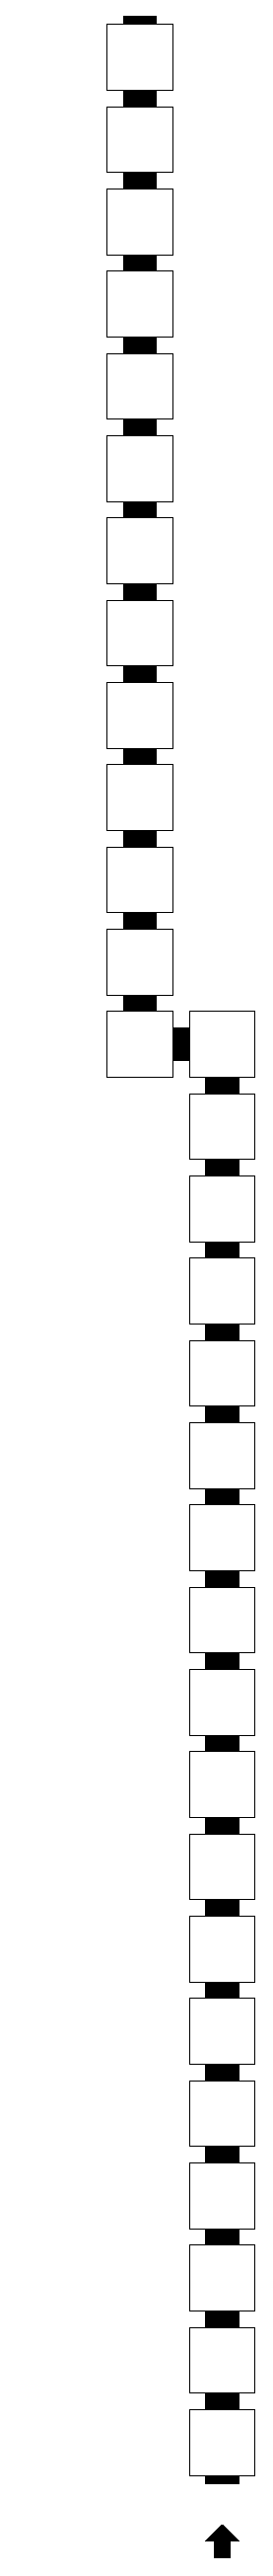
\includegraphics[width=0.2\textwidth]{warping/pre_warp_case1_digit1_msr}
                        \caption{\label{fig:warping/pre_warp_case1_digit1_msr} Case 1 -- Digit 1}
                    \end{subfigure}%
                    ~
                    \begin{subfigure}[t]{0.2\textwidth}
                        \centering
                        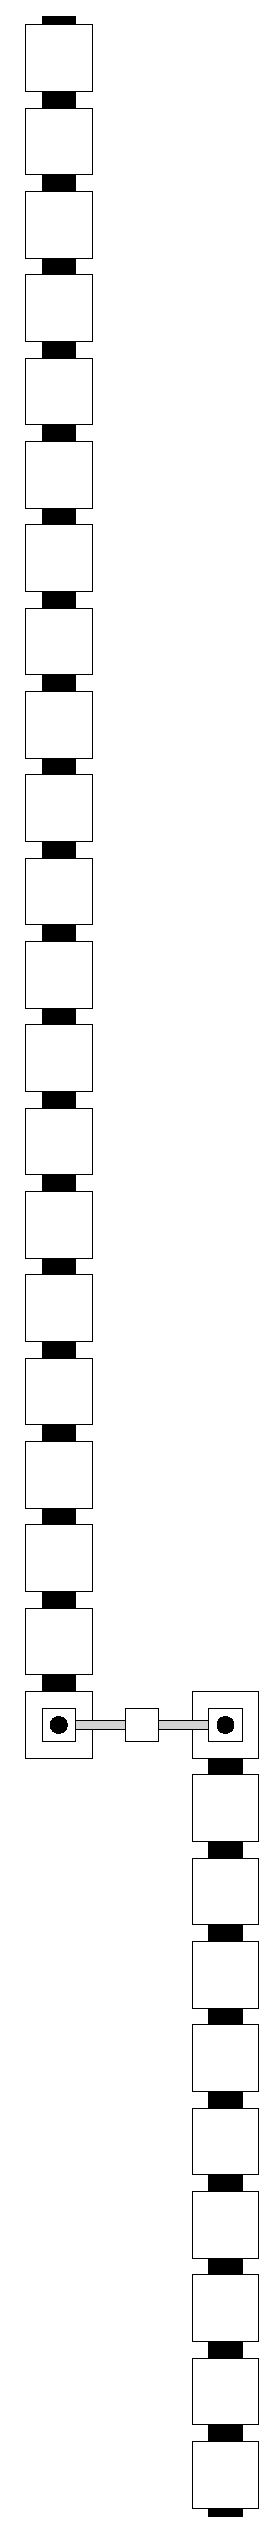
\includegraphics[width=0.2\textwidth]{warping/pre_warp_case2_digit1_msr}
                        \caption{\label{fig:warping/pre_warp_case2_digit1_msr} Case 2 -- Digit 1}
                    \end{subfigure}%
                    ~
                    \begin{subfigure}[t]{0.2\textwidth}
                        \centering
                        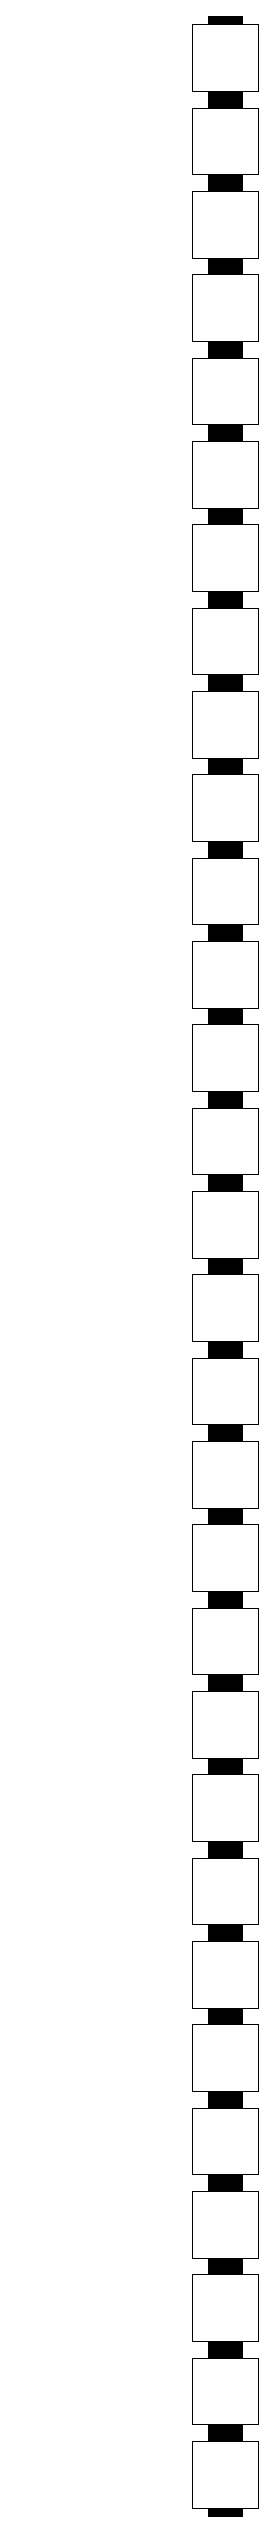
\includegraphics[width=0.2\textwidth]{warping/pre_warp_case2_digit2_msr}
                        \caption{\label{fig:warping/pre_warp_case2_digit2_msr} Case 2 -- Digit 2}
                    \end{subfigure}%
                    ~
                    \caption{\label{fig:pre_warp_gadgets} {\prewarp} gadgets }
                \end{figure}


            \item $\firstwarp (\langle d, i, \inc\rangle)$ $\approx O(1)$
                1 tile is created

            \item $\warpbridge(\langle d, i, \inc\rangle)$ $\approx O(1)$

                A {\warpbridge} gadget binds the last tile of the {\firstwarp} gadgets to the
                first tile of the {\secondwarp} gadgets. In case 1, and case 2 - digit 1, the
                {\warpbridge} is omitted from the {\warpunit}.

                \begin{figure}[H]
                    \begin{subfigure}[t]{0.2\textwidth}
                        \centering
                        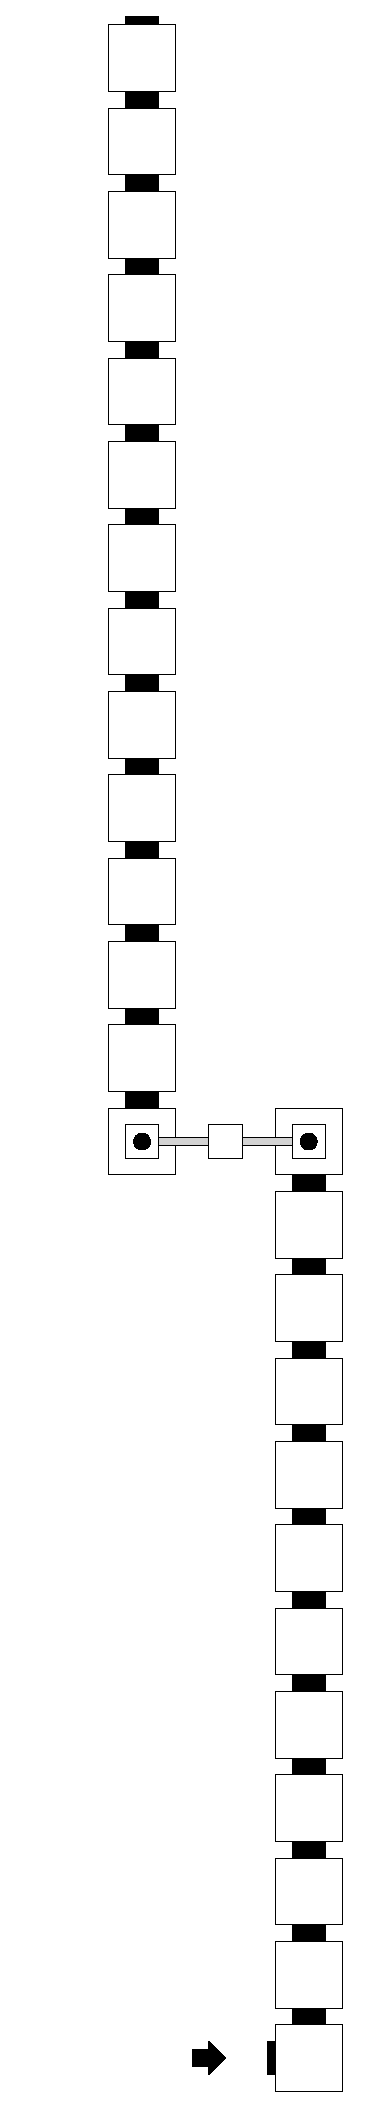
\includegraphics[width=0.2\textwidth]{warping/warp_bridge_general}
                        \caption{\label{fig:warping/warp_bridge_general} General}
                    \end{subfigure}%
                    ~
                    \begin{subfigure}[t]{0.2\textwidth}
                        \centering
                        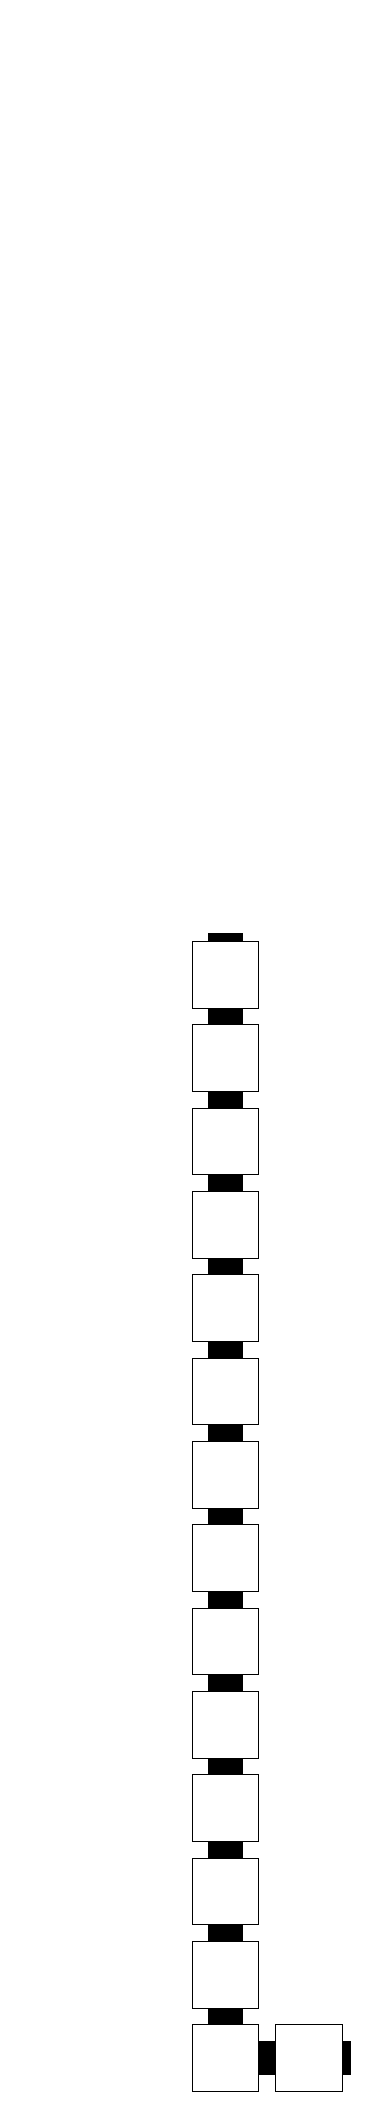
\includegraphics[width=0.2\textwidth]{warping/warp_bridge_case2_digit2_msr}
                        \caption{\label{fig:warping/warp_bridge_case2_digit2_msr} Case 2 -- Digit 2}
                    \end{subfigure}%
                    ~
                \end{figure}

            \item $\secondwarp(\langle d, i, \inc\rangle)$ $\approx O(1)$
                1 tile is created, $O(1)$.

            \item $\postwarp  (\langle d, i, \inc\rangle)$ $\approx O(1)$
                \begin{figure}[H]
                    \begin{subfigure}[t]{0.2\textwidth}
                        \centering
                        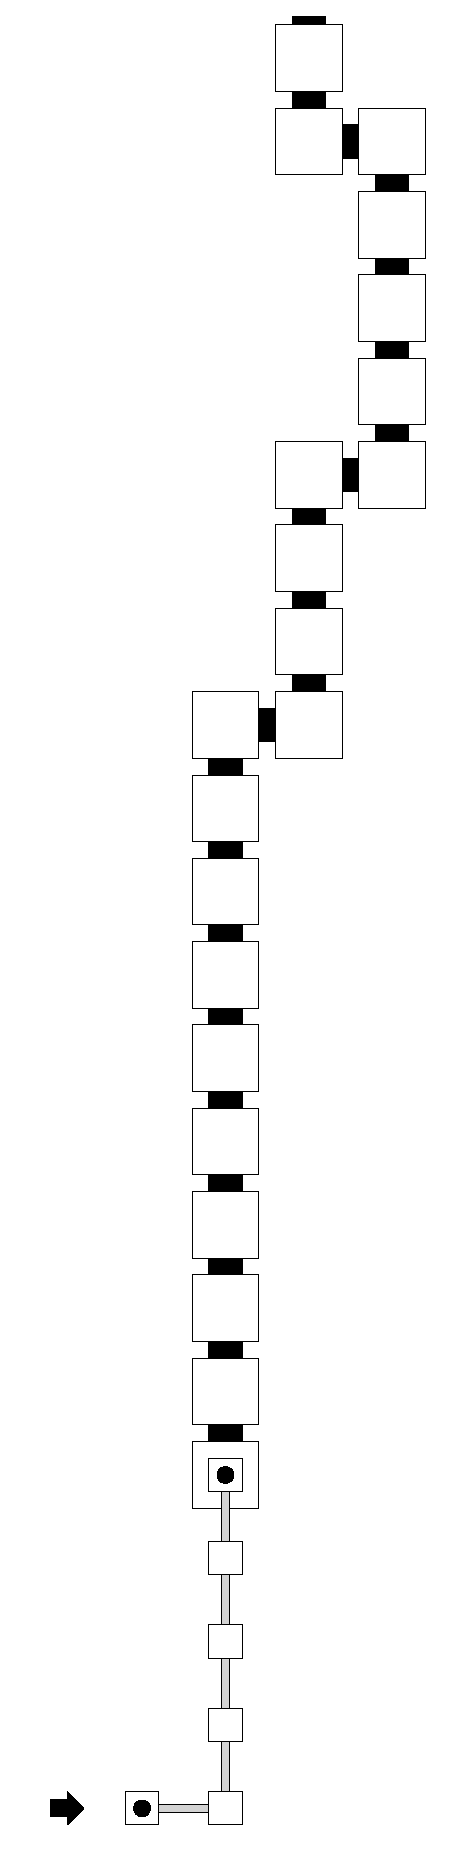
\includegraphics[width=0.2\textwidth]{warping/post_warp_general_digit1}
                        \caption{\label{fig:warping/post_warp_general_digit1} General Digit 1}
                    \end{subfigure}%
                    ~
                    \begin{subfigure}[t]{0.2\textwidth}
                        \centering
                        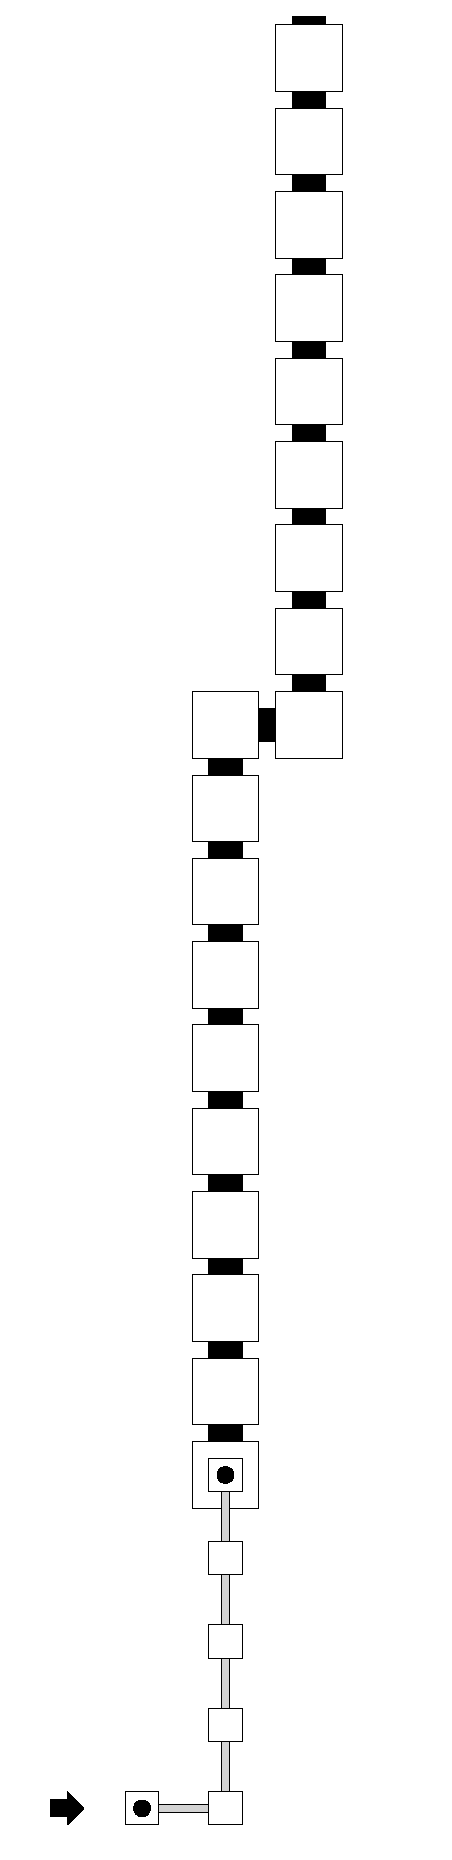
\includegraphics[width=0.2\textwidth]{warping/post_warp_general_digit2and3}
                        \caption{\label{fig:warping/post_warp_general_digit2and3} General Digits 2 and 3 }
                    \end{subfigure}%
                    ~
                    \begin{subfigure}[t]{0.2\textwidth}
                        \centering
                        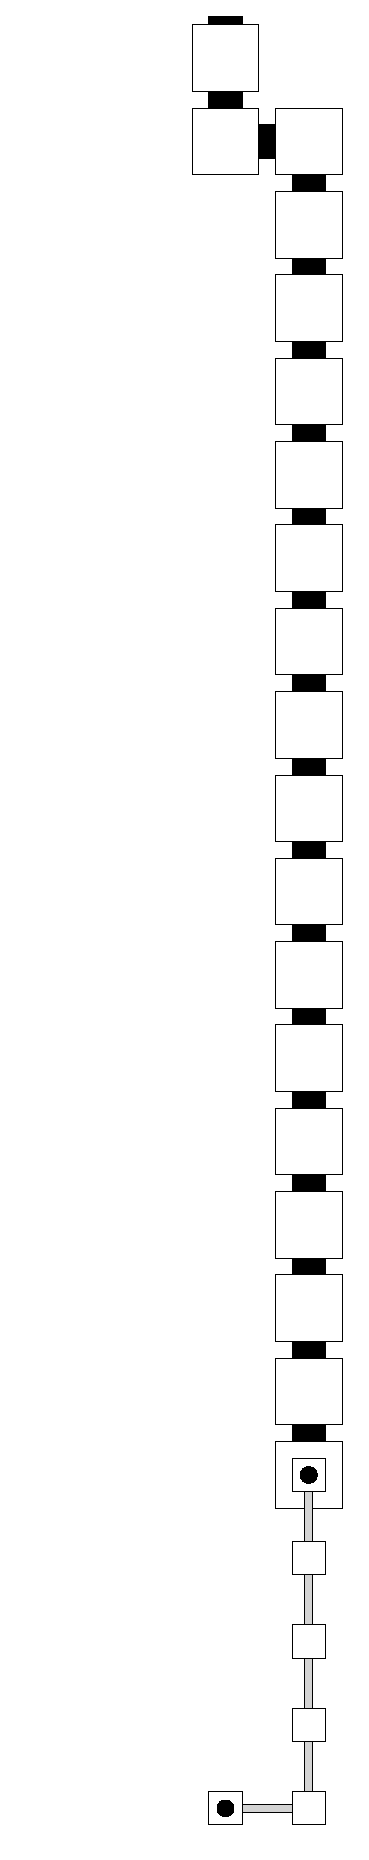
\includegraphics[width=0.2\textwidth]{warping/post_warp_case1_digit1_msr}
                        \caption{\label{fig:warping/post_warp_case1_digit1_msr} Case 1 -- Digit 1}
                    \end{subfigure}%
                    ~
                    \begin{subfigure}[t]{0.2\textwidth}
                        \centering
                        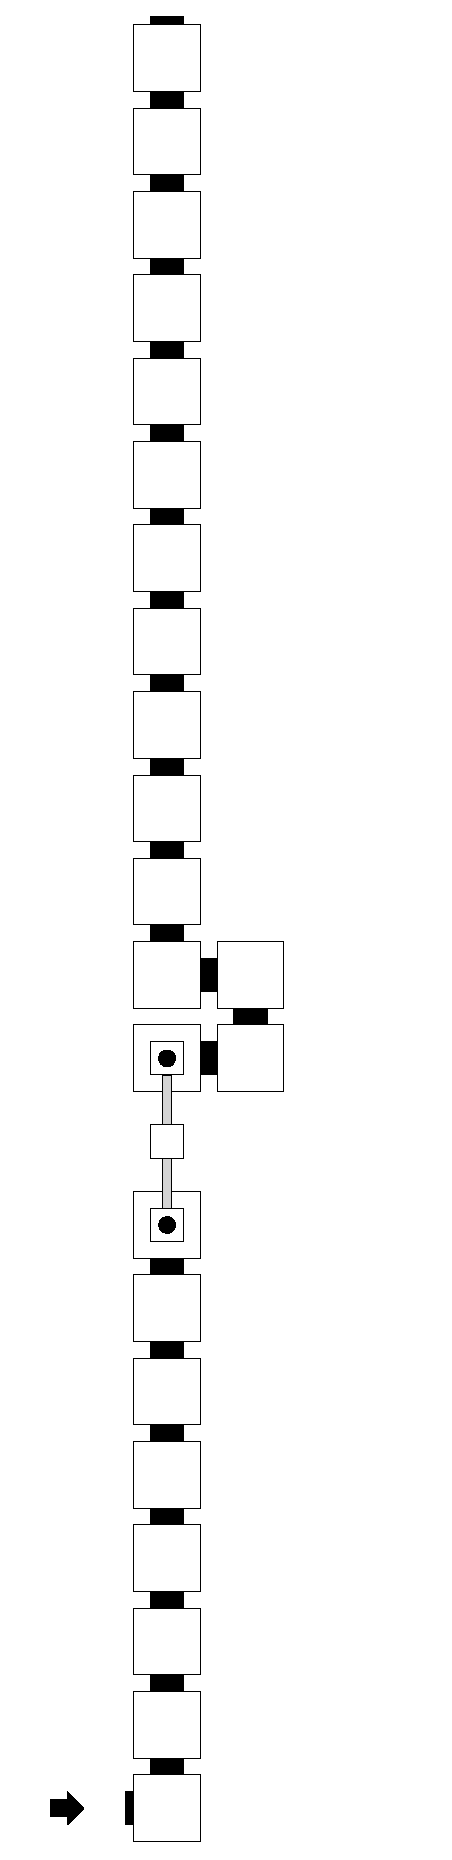
\includegraphics[width=0.2\textwidth]{warping/post_warp_case2_digit1_msr}
                        \caption{\label{fig:warping/post_warp_case2_digit1_msr} Case 2 -- Digit 1}
                    \end{subfigure}%
                    ~

                    \begin{subfigure}[t]{0.2\textwidth}
                        \centering
                        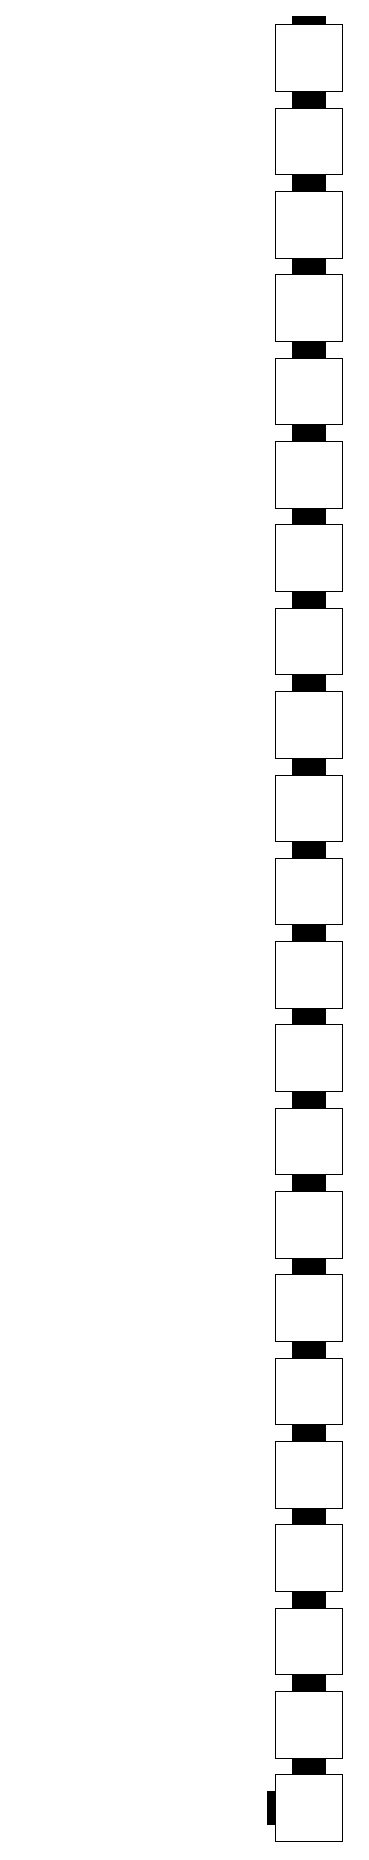
\includegraphics[width=0.2\textwidth]{warping/post_warp_case2_digit2_msr}
                        \caption{\label{fig:warping/post_warp_case2_digit2_msr} Case 2 -- Digit 2}
                    \end{subfigure}%
                    ~
                    \caption{\label{fig:post_warp_gadgets} {\postwarp} gadgets }
                \end{figure}

        \end{enumerate}

        Tiles created for the warp units $\approx O(\log m)$
    % For each digit length L
    \subsubsection{ Digit writers }
        % For each index in 1, 2, 3, and carry in 0,1
        %

    \subsubsection{ Digit tops }
    The {\dtop} gadgets have specific geometry, such that they allow {\firstwarp} and
    {\secondwarp} units to ``wake up" and end their warp journey. A {\dtop} is placed on
    the north end of a digit. These hold a increment/copy signal and the regional index
    of the next digit to read. $\approx O(\log m)$
    \vspace{1cm}

        For each {\inc} $\in \{ {\tt increment, copy } \}$
        \begin{itemize}
            \item General digit tops common to all assemblies

            \begin{enumerate}[label={--}]
                \item create \dtop ($\langle \inc, 1, l \rangle$)
                \begin{flalign*}
                    \text{input$\rightarrow$south}  & = \dtop(\inc, 1) \\
                    \text{output$\rightarrow$south} & = \returnfromdonereaddtwo(\inc)
                \end{flalign*}
                \vspace{.5cm}

                \item create \dtop ($\langle \inc, 2, l \rangle$)
                \begin{flalign*}
                    \text{input$\rightarrow$south}  & = \dtop(\inc, 2) \\
                    \text{output$\rightarrow$south} & = \returnfromdtworeaddthree(\inc)
                \end{flalign*}
                \vspace{.5cm}

                \item create \dtop ($\langle \inc, 3, l \rangle$)
                \begin{flalign*}
                    \text{input$\rightarrow$south}  & = \dtop(\inc, 3) \\
                    \text{output$\rightarrow$south} & = \returnfromdthreereaddone(\inc)
                \end{flalign*}
                \vspace{.5cm}
            \end{enumerate}

        \item MSR-specific digit tops.
            \begin{enumerate}[label={--}]

            % For digit 1, in MSR, in case 2
            \item if $i$ is 1 and MSR contains 2 digits: create $\dtopdonecasetwo(\langle \inc, l \rangle)$
            \begin{flalign*}
                \text{input$\rightarrow$south}  & = \dtopdonecasetwo(\inc) \\
                \text{output$\rightarrow$south} & = \returnfromdonereaddtwocasetwo(\inc)
            \end{flalign*}
            \vspace{.5cm}

            % For digit 2 in case 2, in MSR (MSD)
            \item if $i$ is 2 and MSR contains 2 digits: create $\dtopdtwocasetwo(\langle \inc, l \rangle)$
            \begin{flalign*}
                \text{input$\rightarrow$south}  & = \dtopdtwocasetwo(\inc) \\
                \text{output$\rightarrow$south} & = \returnfromdtworeadnextrow(\inc)
            \end{flalign*}
            \vspace{.5cm}

            % For digit 3, in MSR, in case 3 (MSD)
            \item if $i$ is 3 and MSR contains 3 digits: create $\dtopdthreecasethree(\langle \inc, l \rangle)$
            \begin{flalign*}
                \text{input$\rightarrow$south}  & = \dtopdthreecasethree(\inc) \\
                \text{output$\rightarrow$south} & = \returnfromdthreereadnextrow(\inc)
            \end{flalign*}
            \vspace{.5cm}

        \end{enumerate}
    \end{itemize}

    \subsubsection{Return paths between the MSD and LSD in different rows}
    The gadgets of this class hold a increment/copy signal.
    The height of these gadgets is dependent on $l$ and the width is dependent of $k$.
    These gadgets are used to begin reading the first digit in the following row, once
    the MSD has been read in the current row.
    \vspace{1cm}

    \noindent For each {\inc} $\in \{ {\tt increment, copy } \}$

        \begin{enumerate}
            \item \returnfromdonereadnextrow

            \begin{flalign*}
                \text{input$\rightarrow$south}  & = \returnfromdonereadnextrow(\inc) & \\
                \text{output$\rightarrow$north} & = \dreader(\inc, 1)
            \end{flalign*}
            % $\approx O(\log m) + O(k)$
            \vspace{.5cm}

            \item \returnfromdtworeadnextrow
            \begin{flalign*}
                \text{input$\rightarrow$north}  & = \returnfromdtworeadnextrow(\inc) & \\
                \text{output$\rightarrow$north} & = \dreader(\inc, 1)
            \end{flalign*}
            % $\approx O(\log m) + O(k)$
            \vspace{.5cm}

            \item \returnfromdthreereadnextrow
            \begin{flalign*}
                \text{input$\rightarrow$north}  & = \returnfromdthreereadnextrow(\inc) & \\
                \text{output$\rightarrow$north} & = \dreader(\inc, 1)
            \end{flalign*}
            % $\approx O(\log m) + O(k)$

        \end{enumerate}

    \vspace{1cm}
    \subsubsection{Return paths between digits in the same row}
        The gadgets of this class hold a increment/copy signal and the regional index
        of the next digit to read. The height of these gadgets is dependent on $l$.
        These gadgets are used so that upon writing a digit, the counter
        is able to move back down to the next digit in the current row, and continue
        reading.

        \begin{enumerate}[label={--}]
            \item \returnfromdonereaddtwo
            \begin{flalign*}
                \text{input$\rightarrow$north}  & = \returnfromdonereaddtwo(\inc) & \\
                \text{output$\rightarrow$north} & = \dreader(\inc, 2)
            \end{flalign*}\vspace{.5cm}

            \item \returnfromdonereaddtwocasetwo
            \begin{flalign*}
                \text{input$\rightarrow$north}  & = \returnfromdonereaddtwocasetwo (\inc) & \\
                \text{output$\rightarrow$north} & = \dreader(\inc, 2)
            \end{flalign*}\vspace{.5cm}

            \item \returnfromdtworeaddthree
            \begin{flalign*}
                \text{input$\rightarrow$north}  & = \returnfromdtworeaddthree(\inc) & \\
                \text{output$\rightarrow$north} & = \dreader(\inc, 3)
            \end{flalign*}\vspace{.5cm}


            \item \returnfromdthreereaddone
            \begin{flalign*}
                \text{input$\rightarrow$north}  & = \returnfromdthreereaddone(\inc) & \\
                \text{output$\rightarrow$north} & = \dreader(\inc, 1)
            \end{flalign*}

        \end{enumerate}



\subsection{Seed Unit}

